% !TEX spellcheck = en_US
% !TEX spellcheck = LaTeX
\documentclass[letterpaper,10pt,english]{article}
\usepackage{%
	amsfonts,%
	amsmath,%	
	amssymb,%
	amsthm,%
	babel,%
	bbm,%
	%biblatex,%
	caption,%
	centernot,%
	color,%
	enumerate,%
	%enumitem,%
	epsfig,%
	epstopdf,%
	etex,%
	fancybox,%
	framed,%
	fullpage,%
	%geometry,%
	graphicx,%
	hyperref,%
	latexsym,%
	mathptmx,%
	mathtools,%
	multicol,%
	pgf,%
	pgfplots,%
	pgfplotstable,%
	pgfpages,%
	proof,%
	psfrag,%
	%subfigure,%	
	tikz,%
	times,%
	ulem,%
	url,%
	xcolor,%
	mathpazo
}

\definecolor{shadecolor}{gray}{.95}%{rgb}{1,0,0}
\usepackage[margin=1in,top=0.75in]{geometry}
\usepackage[mathscr]{eucal}
\usepgflibrary{shapes}
\usepgfplotslibrary{fillbetween}
\usetikzlibrary{%
  arrows,%
  backgrounds,%
  chains,%
  decorations.pathmorphing,% /pgf/decoration/random steps | erste Graphik
  decorations.text,% 
  matrix,%
  positioning,% wg. " of "
  fit,%
  patterns,%
  petri,%
  plotmarks,%
  scopes,%
  shadows,%
  shapes.misc,% wg. rounded rectangle
  shapes.arrows,%
  shapes.callouts,%
  shapes%
}

%\pgfplotsset{compat=newest} %<------ Here
\pgfplotsset{compat=1.11} %<------ Or use this one

\theoremstyle{plain}
\newtheorem{thm}{Theorem}[section]
\newtheorem{lem}[thm]{Lemma}
\newtheorem{prop}[thm]{Proposition}
\newtheorem{cor}[thm]{Corollary}
\newtheorem{clm}[thm]{Claim}

\theoremstyle{definition}
\newtheorem{axiom}[thm]{Axiom}
\newtheorem{defn}[thm]{Definition}
\newtheorem{conj}[thm]{Conjecture}
\newtheorem{exmp}[thm]{Example}
\newtheorem{exerc}[thm]{Exercise}
\newtheorem{assum}[thm]{Assumptions}

\theoremstyle{remark}
\newtheorem{rem}[thm]{Remark}
\newtheorem{note}[thm]{Note}

\newcommand{\Cov}{\operatorname{Cov}}
%\newcommand{\det}{\operatorname{det}}
\newcommand{\Real}{\mathbb{R}}
\newcommand{\tr}{\operatorname{tr}}
%\newcommand{\Var}{\operatorname{Var}}

\DeclareMathOperator{\sign}{sign}
%\renewcommand{\proof}[1]{\begin{proof}#1\end{proof}}
\newcommand{\EQ}[1]{\begin{equation*}#1\end{equation*}}
\newcommand{\EQN}[1]{\begin{equation}#1\end{equation}}
\newcommand{\eq}[1]{\begin{align*}#1\end{align*}}
\newcommand{\meq}[2]{\begin{xalignat*}{#1}#2\end{xalignat*}}
\newcommand{\norm}[1]{\left\lVert#1\right\rVert}
\newcommand{\abs}[1]{\left\lvert#1\right\rvert}
\newcommand{\expect}[1]{\mathbb{E}\left[{#1}\right]}
\newcommand{\prob}[1]{\mathbb{P}\left[{#1}\right]}
\newcommand{\given}{\; \big\vert \;} 
\newcommand{\set}[1]{\left\{#1\right\}} 
\newcommand{\indicator}[1]{\mathbb{1}_{\set{#1}}} 
\newcommand{\inner}[1]{\left\langle#1\right\rangle}
\newcommand{\red}[1]{\textcolor{red}{#1}} 
\newcommand{\E}[1]{\mathbb{E}\left[#1\right]}
\newcommand{\Var}[1]{\operatorname{Var}\left[#1\right]}

\newcommand{\D}{\mathbb{D}}
%\newcommand{\E}{\mathbb{E}}
\newcommand{\N}{\mathbb{N}}
\renewcommand{\P}{\mathbb{P}}
\newcommand{\Q}{\mathbb{Q}}
\newcommand{\R}{\mathbb{R}}
\newcommand{\Z}{\mathbb{Z}}

\newcommand{\bU}{\mathbf{1}}
\newcommand{\bx}{\mathbf{x}}

\newcommand{\cB}{\mathcal{B}}
\newcommand{\cC}{\mathcal{C}}
\newcommand{\cD}{\mathcal{D}}
\newcommand{\cF}{\mathcal{F}}
\newcommand{\cG}{\mathcal{G}}
\newcommand{\cH}{\mathcal{H}}
\newcommand{\cO}{\mathcal{O}}
\newcommand{\cT}{\mathcal{T}}
\newcommand{\cX}{\mathcal{X}}
\newcommand{\cY}{\mathcal{Y}}

\newcommand{\sA}{\mathscr{A}}
\newcommand{\sB}{\mathscr{B}}
\newcommand{\sC}{\mathscr{C}}
\newcommand{\sD}{\mathscr{D}}
\newcommand{\sE}{\mathscr{E}}
\newcommand{\sF}{\mathscr{F}}
\newcommand{\sG}{\mathscr{G}}
\newcommand{\sH}{\mathscr{H}}
\newcommand{\sL}{\mathscr{L}}
\newcommand{\dO}{\mathscr{O}}
\newcommand{\sS}{\mathscr{S}}
\newcommand{\sT}{\mathscr{T}}
\newcommand{\sX}{\mathscr{X}}
\newcommand{\sY}{\mathscr{Y}}
\newcommand{\sZ}{\mathscr{Z}}

% Debug
\newcommand{\todo}[1]{\begin{color}{blue}{{\bf~[TODO:~#1]}}\end{color}}

% a few handy macros

\renewcommand{\le}{\leqslant}
\renewcommand{\ge}{\geqslant}
\newcommand\matlab{{\sc matlab}}
\newcommand{\goto}{\rightarrow}
\newcommand{\bigo}{{\mathcal O}}
%\newcommand{\half}{\frac{1}{2}}
%\newcommand\implies{\quad\Longrightarrow\quad}
\newcommand\reals{{{\rm l} \kern -.15em {\rm R} }}
\newcommand\complex{{\raisebox{.043ex}{\rule{0.07em}{1.56ex}} \hskip -.35em {\rm C}}}


% macros for matrices/vectors:

% matrix environment for vectors or matrices where elements are centered
\newenvironment{mat}{\left[\begin{array}{ccccccccccccccc}}{\end{array}\right]}
\newcommand\bcm{\begin{mat}}
\newcommand\ecm{\end{mat}}

% matrix environment for vectors or matrices where elements are right justifvied
\newenvironment{rmat}{\left[\begin{array}{rrrrrrrrrrrrr}}{\end{array}\right]}
\newcommand\brm{\begin{rmat}}
\newcommand\erm{\end{rmat}}

% for left brace and a set of choices
%\newenvironment{choices}{\left\{ \begin{array}{ll}}{\end{array}\right.}
\newcommand\when{&\text{if~}}
\newcommand\otherwise{&\text{otherwise}}
% sample usage:
%  \delta_{ij} = \begin{choices} 1 \when i=j, \\ 0 \otherwise \end{choices}


% for labeling and referencing equations:
\newcommand{\eql}{\begin{equation}\label}
\newcommand{\eqn}[1]{(\ref{#1})}
% can then do
%  \eql{eqnlabel}
%  ...
%  \end{equation}
% and refer to it as equation \eqn{eqnlabel}.  


% some useful macros for finite difference methods:
\newcommand\unp{U^{n+1}}
\newcommand\unm{U^{n-1}}

% for chemical reactions:
\newcommand{\react}[1]{\stackrel{K_{#1}}{\rightarrow}}
\newcommand{\reactb}[2]{\stackrel{K_{#1}}{~\stackrel{\rightleftharpoons}
   {\scriptstyle K_{#2}}}~}


\makeatletter
\def\th@plain{%
  \thm@notefont{}% same as heading font
  \itshape % body font
}
\def\th@definition{%
  \thm@notefont{}% same as heading font
  \normalfont % body font
}
\makeatother
\date{}

\graphicspath{{Figures/}}
\title{Lecture-22: Boltzmann Machines}
\author{}

\begin{document}
	

	
	
	
	%%%%%%%%%%%%%%%%%%%%%%%%%%%%%%%%%%
\maketitle
Restricted Boltzmann machine (RBM) is a type of artificial neural network (ANN), capable of dimensionality reduction, feature learning and clasification. In this lecture we give a short introduction about artificial neural networks and restricted boltzmann machines (RBMs), then we derive some interesting properties of RBMs.\\

% section 1
\section{Artificial Neural Network (ANN)}
Artificial neural network is a computing framework, based on biological brain architecture, which tries to mimic human's ability to learn from experience (called training examples).\\
\begin{enumerate}
	% sub-section
	\item \textbf{Architecture} It is large network of interconnected units called artificial neurons.
	It has a simple input-output mapping: computing output based on weighted sum of the received signal(s), and associated bias. The weight of the input signal(s) can be interpreted as the strength of the respective connection which varies from $0$ to $1$ (with $0$ implying that the signal does not affect the neuron's computation). The output of this neuron would in turn affect its downstream neurons. Usually the edges are directed.\\
	Usually groups of neurons aggregate together in layers: 
	\begin{enumerate}
		\item Visible layer: Aggregate of Input nodes
		\item Hidden layer(s):  Aggregate of nodes associated with computation
		\item Output layer:  Aggregate of output nodes
	\end{enumerate}
	% sub-section
	\item \textbf{Computation} Output (or state) of a single neuron is represented by
	\begin{center} $ x =\sigma(\sum_{i=1}^d w_i x_i +b)$,
		where $\sigma(u)=\frac{1}{1+e^{-u}}$ is the sigmoid function.
	\end{center}
	% sub-section
	\item \textbf{Learning} Learning in artificial neuron network would correspond to estimating the model parameters (the edge weights and biases) according to the training examples (explained later).
\end{enumerate}

% section 2
\section{Boltzmann Machine (BM)}
Boltzmann machine is used for unsupervised learning. In this neural network, there is a layer of visible nodes and a layer of hidden nodes, and the connections are undirected. During implementation, the Boltzmann distribution is used for sampling, hence the name.
\begin{enumerate}
	% sub-section
	\item \textbf{As a recurrent Markov Chain} Suppose we digitize the state of the $j^{th}$ neuron as\\
	\begin{center}
		$ x_{j}=
		\begin{cases}
		1 & \text{if }\sum_{i=1, i\neq j}^d w_{ij} x_i +b_j \geq 0\\
		0 & \text{otherwise}
		\end{cases}
		$
	\end{center}
	Suppose we denote the state of BM, $X$, as configuration of all the neurons, $X = (x_{1}, x_{2}, \ldots x_{d})$. Thus, given the current state of the BM, as well as the  model parameters (the edge weights and biases), we can relay the signal of each neuron to its connected neurons and compute state of each neurons. So the Boltzmann machine can be viewed as a Markov Chain.
	
	% sub-section
	\item \textbf{Learning} Given the weights and biases, the flow of signal is determined and a steady state will be reached. Analyzing the examples the aim of learning is to modify the model parameters such that the model/framework tries to mimic the distribution of the training example.\\
	Initialize the model parameters randomly.
	\begin{enumerate}
		\item Initialize the visible nodes of BM according to the example, and hidden nodes as zero.
		\item Allow the network to reach steady state
		\item Compare the state of visible nodes with the example.
		\item Modify the model parameters such that the above difference is minimized.
	\end{enumerate}
	Thus, we would like to maximize the probabilty function (of steady state of BM) corresponding to the training example. So if an energy function for the global state of BM was defined, we would try to minimize it for the configuration corresponding to the training example.
	Probability function, $$P(X)=\frac {e^{-E(X)}}{Z} \text{, and energy function, } , E(X)=-X^TUX-B^TX,$$ where Z is the partition function that ensures that $\sum_XP(X)=1$ and $X = (x_{1}, x_{2}, \ldots, x_{d})$ is the state vector, $U$ is the "weight" matrix of model parameters and $B$ is the vector of bias parameters.\\
	% sub-section
	\item \textbf{Energy function} 
	The state of the boltzmann machine, \textbf{$X$}, can be divided into layer of visible nodes (\textbf{$v$}) and layer of hidden nodes (\textbf{$h$}), i.e. $\textbf{$X$} = (\textbf{v}, \textbf{h})$.\\
	$$ E(X)=-X^TUX-B^TX \\
	\implies E(v,h)=-v^TRv-v^TWh-h^TSh-b^Tv-c^Th$$\\
	where $R$, $W$ and $S$ are the weight sub-matrices corresponding to visible-visible, visible-hidden and hidden-hidden connections, respectively, and $b$ and $c$ are the bias vector associated to neurons of visible layer and of hidden layer respectively.
	
	% sub-section
	\textbf{Some considerations}
	Theoretically Boltzmann machines are very powerful specially useful when not all the variables (visible nodes) are observed. In this case, the unobserved variables can act similarly to hidden units in a multilayer perceptron and model higher-order interactions among the visible units. Boltzmann machine with hidden units becomes a universal approximator of probability mass functions over discrete variables. Such machines hence would be useful for example in recommender system (the Netflix Challenge), to complete partial images.
	Evaluation of partition function for boltzmann machines is intractable. Additionally, the time complexity of learning in a general, unconstrained Boltzmann machine, grows exponentially with its size. Hence its implementation is  impractical even for a small sized machine.
	
	However by constraining the allowed connection in a Boltzmann machine, the learning can be made efficient enough for practical purpose. This is discussed in the next section.
\end{enumerate}

% section 3
\section{Restricted Boltzmann Machine (RBM)}
In Restricted Boltzmann Machines, intra-layer connections are not allowed. The network thus reduces to a bi-partite graph. Each neuron of a particular layer is independent of other neurons of that layer.
Let the observed layer consist of a set of $n_v$ binary random variables (corresponding to state of the visible neurons), which we refer to collectively with the vector \textbf{$v$}. We refer to the latent or hidden layer of $n_h$ binary random variables (corresponding to state of the visible neurons) as \textbf{$h$}.\\
Global state, 	$X = (v, h)$.\\
Visible layer,	$v = (v_{1}, v_{2}, \ldots, v_{n_v})$.\\
Hidden layer,	$h = (h_{1}, h_{2}, \ldots, h_{n_h})$.\\
Example: Movie recommendation is good example of RBM. At visible nodes differnt movies are given and hidden layer learns different properties like Genre, Actor, Award etc.


\begin{enumerate}
	% sub-section
	\item \textbf{Energy function} Like the general Boltzmann machine, the restricted Boltzmann machine is an energy-based model with the joint probability distribution specified by its energy function.
	$$P(\textbf{v}={v},\textbf{h}=h)=\frac{1}{Z}e^{-E(v,h)}$$ where $E$ denotes the energy function and $Z=\sum_v \sum_h e^{-E(v,h)}$ is the partition function. Since intra-layer connections are not allowed, the energy function, $E$, is given by\\
	$E(v,h)=-b^Tv-c^Th-v^TWh$\\
	$\implies E(v,h)=-\sum_{i=1}^{n_v}b_iv_i-\sum_{j=1}^{n_h}c_jh_j-\sum_{i=1}^{n_v}\sum_{j=1}^{n_h}v_iW_{ij}h_j$.\\
	
	\textbf{Reducing energy} We observe that
	\begin{enumerate}
		\item If a particular pair of visible node, $v_{i}$ and hidden node, $h_{j}$ are to be associated, then increasing the weight of the edge connecting them, $w_{ij}$, should reduce the energy and thus the association will be learned.
		\item If a particular node is activated often in the series of training examples, increase in bias for that node would reduce the energy and thus is favourable.
	\end{enumerate}
	In the following we would formalize the above, and derive some interesting properties of Restricted Boltzmann Machine.
	
	
\end{enumerate}







\begin{figure}
	\centering
	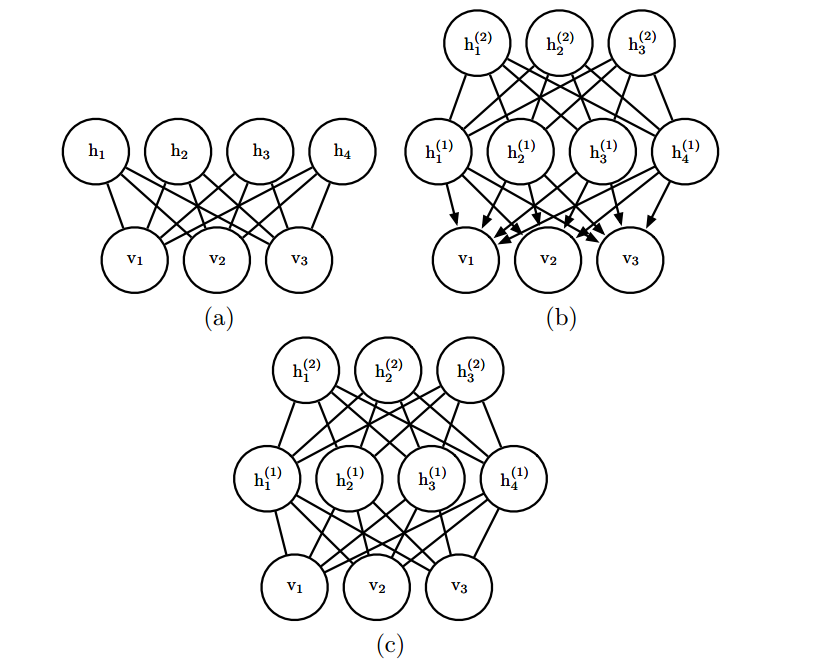
\includegraphics[scale = 0.4]{machines.png}
	\caption{(a) Restricted boltzmann machine (b) Deep beleif network (c) Deep boltzmann machine}
\end{figure}

\subsection{Conditional Distributions}
Though $P(v)$ is intractable, the bipartite graph structure of the RBM has the
special property of its conditional distributions $P(h|v)$ and $P(v|h)$ being
factorial and relatively simple to compute and sample from.
\begin{align}
P(h|v)&=\frac{P(h,v)}{P(v)}\\
&=\frac{1}{P(v)}\frac{1}{Z}e^{b^Tv+c^Th+v^TWh}\\&=\frac{1}{Z'}e^{c^Th+v^TWh}\\
&=\frac{1}{Z'}e^{\sum_{j=1}^{n_h} c_jh_j+\sum_{j=1}^{n_h} v^TW_{:,j}hj}\\
&=\frac{1}{Z'}\prod_{j=1}^{n_h}e^{c_jh_j+v^TW_{:,j}h_j}.
\end{align}
Where $W_{:,j}$ is $j^th$ column of W.
\begin{align}
P(h_j=1|v)&=\frac{\widetilde{P}(h_j=1|v)}{\widetilde{P}(h_j=0|v)+\widetilde{P}(h_j=1|v)}\\
&=\frac{e^{c_j+v^TW_{:,j}}}{e^0+e^{c_j+v^TW_{:,j}}}\\
&=\sigma(c_j+v^TW_{:,j})\\
P(h_j=0|v)&=\sigma(-(c_j+v^TW_{:,j}))
\end{align}

Full conditional over the hidden layer as factorial distribution is given by
$$P(h|v)=\prod_{j=1}^{n_h}\sigma((c_j+W_{:,j}^Tv)(2h_j-1))$$
Similarly $$P(v|h)=\prod_{i=1}^{n_v}\sigma((b_i+W_{i,:}h)(2v_i-1))$$

\subsection{Traning RMB}
The log-likelihood is given by
\begin{align}
l(W,b,c)&=\sum_{t=1}^n logP(v^{(t)})\\
&=\sum_{t=1}^n log\sum_hP(v^{(t)},h)\\
&= \sum_{t=1}^n log\sum_h \frac{1}{Z}e^{-E(h,v)}\\
&= \sum_{t=1}^n log\sum_h e^{-E(v^{(t)},h)}-nlogZ\\
&=\sum_{t=1}^n log\sum_h e^{-E(v^{(t)},h)}-nlog\sum_{v,h}e^{-E(v,h)}
\end{align}
Let $\theta={b,c,W}$, For learning maximize the log likelihood 
\begin{align}
l(\theta)&=\sum_{t=1}^n log\sum_h e^{-E(v^{(t)},h)}-nlog\sum_{v,h}e^{-E(v,h)}\\ 
\nabla_{\theta}l(\theta)&=\nabla_\theta \sum_{t=1}^n log\sum_h e^{-E(v^{(t)},h)}-n \nabla_\theta log\sum_{v,h}e^{-E(v,h)}\\
&=\sum_{t=1}^n \frac{\sum_h e^{-E(v^{(t)},h)}\nabla_\theta (-E(v^{(t)},h))}{\sum_h e^{-E(v^{(t)},h)}} -n\frac{\sum_{v,h}e^{-E(v,h)}\nabla_\theta (-E(v,h))}{\sum_{v,h} e^{-E(v,h)}}\\
&=\sum_{t=1}^n \mathbb{E}_{P(h|v^{(t)})}\nabla_\theta (-E(v^{(t)},h))- n\mathbb{E}_{P(v,h)}\nabla_\theta (-E(v,h))
\end{align}
\begin{align}
\nabla_W(-E(v,h))=hv^T\\
\nabla_b(-E(v,h))=v\\
\nabla_c(-E(v,h))=h
\end{align}
Update rules for gradient ascent are given by
\begin{align}
\nabla_Wl(W,b,c)=\sum_{t=1}^n \hat{h}^{(t)}v^{(t)T}-n \mathbb{E}_{P(v,h)}[hv^T]\\
\nabla_bl(W,b,c)=\sum_{t=1}^n v^{(t)T}-n \mathbb{E}_{P(v,h)}[v]\\
\nabla_cl(W,b,c)=\sum_{t=1}^n \hat{h}^{(t)}-n \mathbb{E}_{P(v,h)}[h]
\end{align}
Where $\hat{h}^{(t)}=\mathbb{E}_{P(h,v^{(t)})}[h]=\sigma(c+v^{(t)}W)$\\

In this case, we can interpret the first term(positive
phase) as pushing down on the energy of training examples and the second term(negative phase)
as pushing up on the energy of samples drawn from the model. It is intractable to compute second term so contrastive divergence is used for second term.\\
\textbf{Contrastive Divergence}:
\begin{itemize}
	\item Replace the expectation by a point estimate at $\tilde{v}$
	\item start sampling chain at $v^{(t)}$ and obtain the point $\tilde{v}$ by Gibbs sampling
\end{itemize}


$$\mathbb{E}_{P(v,h)}\nabla_\theta (-E(v,h)) \approx \nabla_\theta (-E(v,h))|_{v=\tilde{v},h=\tilde{h}} $$


\section{Deep Belief Networks}
The connections between the top two layers
are undirected. The connections between all other layers are directed, with the
arrows pointed toward the layer that is closest to the data.  Today, deep belief
networks have mostly fallen out of favor and are rarely used, but they are still deservedly
recognized for their important role in deep learning history.

\section{Deep Boltzmann Machines}
A Deep Boltzmann machine unlike the Deep belief network (DBN), it is an entirely undirected model. Like the RBM, within each layer,
each of the variables are mutually independent, conditioned on the variables in
the neighboring layers. A deep Boltzmann machine with one visible layer, v, and three hidden layers,
h(1), h(2), and h(3), the joint probability is given by
$$P(v,h^{(1)},h^{(2)},h^{(3)})=\frac{1}{Z(\theta)}e^{-E(v,h^{(1)},h^{(2)},h^{(3)};\theta)}$$
To simplify we omit the bias parameter below
$$E(v,h^{(1)},h^{(2)},h^{(3)};\theta)=-v^TW^{(1)}h^{(1)}-h^{(1)T}W^{(2)}h^{(2)}-h^{(2)T}W^{(3)}h^{(3)}$$
the DBM layers
can be organized into a bipartite graph, with odd layers on one side and even layers
on the other. When we condition on the variables in
the even layer, the variables in the odd layers become conditionally independent.\\
The bipartite structure of the DBM means that we can apply the same
equations we have previously used for the conditional distributions of an RBM
to determine the conditional distributions in a DBM.
In two hidden layers, the activation probabilities are given by
$$P(v_i=1|h^{(1)})=\sigma(W_{i,:}^{(1)}h^{(1)})$$
$$P(h_i^{(1)}=1|v,h^{(2)})=\sigma(v^TW_{:,i}^{(1)}+W_{i,:}^{(2)}h^{(2)})$$
$$P(h_k^{(2)}=1|h^{(1)})=\sigma(h^{(1)}W_{:,k}^{(2)})$$
The bipartite structure makes Gibbs sampling in a deep Boltzmann machine
efficient. The naive approach to Gibbs sampling is to update only one variable
at a time. One might naively assume
that a DBM with l layers requires l + 1 updates, with each iteration updating
a block consisting of one layer of units. Instead, it is possible to update all the
units in only two iterations. Gibbs sampling can be divided into two blocks of
updates, one including all even layers (including the visible layer) and the other
including all odd layers. 
\begin{figure}
	\centering
	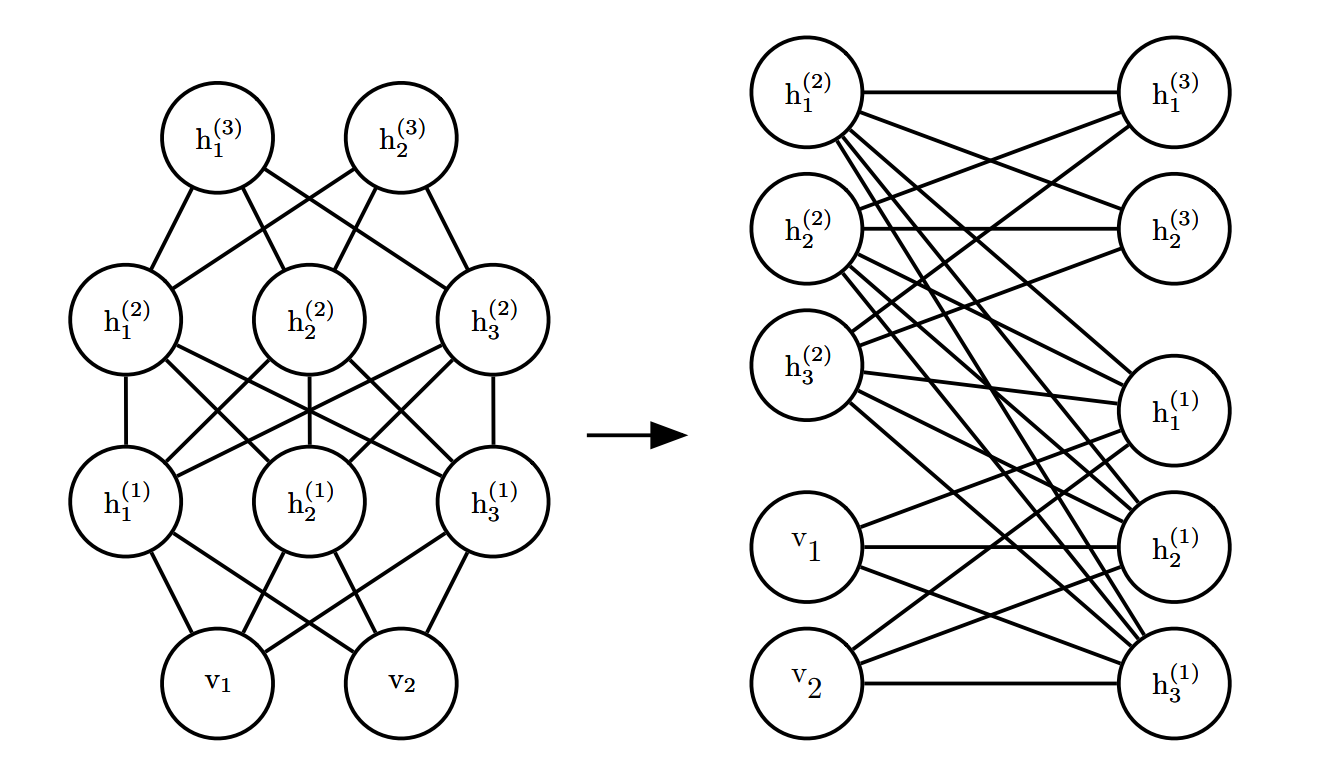
\includegraphics[scale = 0.2]{dbm.png}
	\caption{Rearranged to reveal biparite graph structure}
\end{figure}
\end{document}